
%----------------------------------------------------------------------------------------
%	PACKAGES AND OTHER DOCUMENT CONFIGURATIONS
%----------------------------------------------------------------------------------------

\documentclass{beamer}

\usetheme[hideothersubsections]{Goettingen}
\usepackage{algorithm}
\usepackage{algpseudocode}
\usepackage{graphicx}
\usepackage{subcaption}
\usepackage{amsmath}
\usepackage{amsthm}

% Declare theorem style and numbering
\theoremstyle{plain}
\newtheorem{thm}{Theorem}
\newtheorem{lem}{Lemma}
\newtheorem{corr}{Korrolar}
\theoremstyle{definition}
\newtheorem{defn}[thm]{Definition}
\newtheorem{ex}[thm]{Beispiel}

\newcommand{\mat}[1]{\mathbf{#1}}
\DeclareMathOperator*{\argmax}{arg\,max}
\DeclareMathOperator*{\argmin}{arg\,min}
\newcommand{\norm}[1]{\left\lVert #1 \right\rVert}

%----------------------------------------------------------------------------------------
%	BEGIN DOCUMENT
%----------------------------------------------------------------------------------------


\begin{document}

\title{Sparse Principal Component Analysis}
\subtitle{for Frequency Data}   
\institute{Institute for Numerical Simulation}
\author{Tobias Bork} 
\date{\today}
\titlegraphic{	\vspace{0.5cm}
				
\includegraphics[scale=0.04]{figures/university_of_bonn.png} 				\hspace{1cm}
				
\includegraphics[scale=0.10]{figures/fraunhofer_scai.png}}

\begin{frame}
\titlepage
\end{frame}

%\begin{frame}
%\frametitle{Table of Contents}
%\tableofcontents
%\end{frame}

%----------------------------------------------------------------------------------------
%	Introduction
%----------------------------------------------------------------------------------------

\section{Introduction} 
\begin{frame}
\frametitle{Dimensionality Reduction} 

\begin{itemize}
\item What are DR methods?
\item Why are DR methods important / what is the goal of DR methods?
\item When to use DR methods?

\end{itemize}
\end{frame}

%----------------------------------------------------------------------------------------
%	Principal Component Analysis
%----------------------------------------------------------------------------------------

\section{PCA} 
\subsection{Idea}
\begin{frame}\frametitle{Central Idea}
\begin{itemize}
\item Reduce dimensionality of a data set while retaining as much information as possible
\item extract the most important information from the data table;
\item compress the size of the data set by keeping only this important information;
\item simplify the description of the data set; and
\item analyze the structure of the observations and the variables
\item first component has most variance 
\end{itemize} 
\end{frame}

\begin{frame}
\begin{figure}
\centering
	\begin{subfigure}{0.45\textwidth}
	\centering
	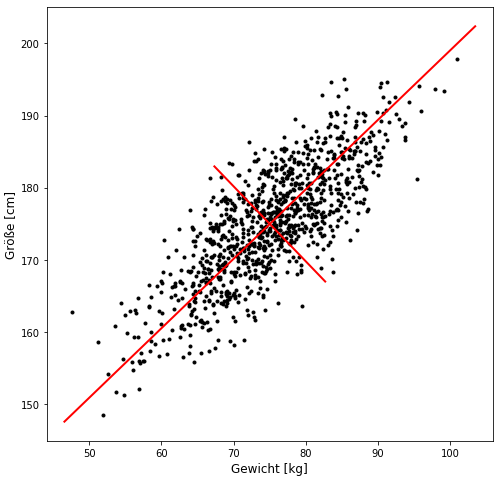
\includegraphics[width = \textwidth]{figures/pca_example.png}
	\label{pca_example_original}
	\end{subfigure}
	%	
	\begin{subfigure}{0.45\textwidth}
	\centering
	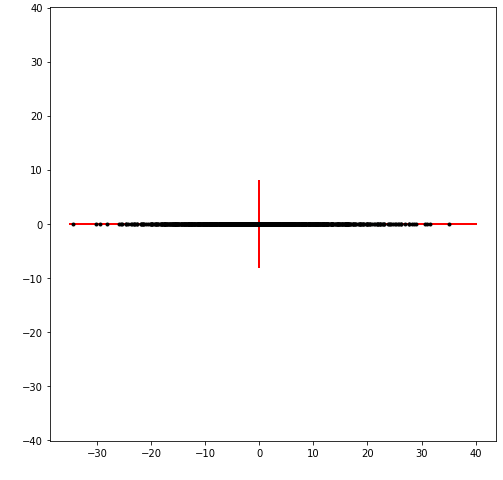
\includegraphics[width = \textwidth]{figures/pca_example_rotated.png}
	\label{pca_example_rotated}
	\end{subfigure}

\caption{Some description of the plots}
\label{pca_example}
\end{figure}
\end{frame}

\subsection{Mathematical Formulations}
\begin{frame}
\frametitle{Mathematical Formulation}
Let $\mat X \in \mathbb{R}^{n \times p}$ be a centered data matrix with $n$ samples and $p$ variables. We find the first principal axis by 
$$v_1 = \argmax_{\norm{v}_2 = 1} \text{Var}[\mat{X}v] = \argmax_{\norm{v}_2 = 1} v^T \mat{\Sigma} v$$
where $\mat{\Sigma} = \mat X^T \mat X$ is the sample covariance matrix.
Then we can find the following principal axis successively
$$v_{k+1} = \argmax_{\norm{v} = 1} v^T \mat{\Sigma} v$$ 
$$\text{subject to }v_{k+1}^Tv_l = 0 \quad \forall 1 \leq l \leq k$$
The new, transformed variables are defined by $Z_i = \mat{X}v_i$

\end{frame}

\begin{frame}
The principal axis can also be computed via the eigendecomposition of $\mat{\Sigma}$.
$$\mat{\Sigma} = \mat V \mat L \mat{V}^T$$
where $\mat{L}$ is a diagonal matrix with eigenvalues $\lambda_i$ and $\mat V$ is the matrix of eigenvectors.
Closely related is the Singular Value Decomposition (SVD) 
$$ \mat{X} = \mat{U}\mat{D}\mat{V}^T $$
where $\mat{D}$ is a diagonal matrix with singular values $d_1,\ldots,d_p$, $\mat{U}$ a $n \times p$ and $\mat{V}$ a $p \times p$ orthogonal matrix.
\end{frame}

\begin{frame}
\frametitle{PCA as a regression problem}
\begin{figure}
\centering
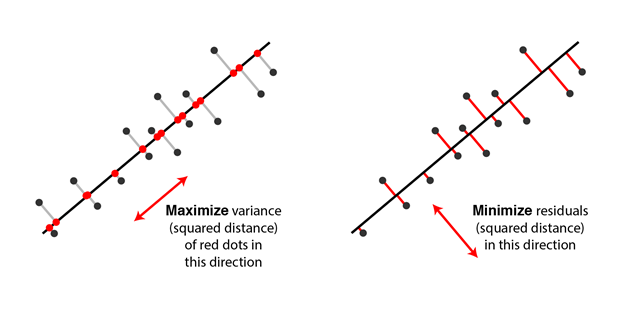
\includegraphics[width = 0.8\textwidth]{figures/pca_projection_explanation.png}
\label{pca_projection_explanation}
\end{figure}
Suppose we want to extract the first $k$ principal axis.
$$\mat{\hat{V}}_k = \argmin_{\mat{V}_k} \sum_{i=1}^{n} \norm{x_i - \mat{V}_k \mat{V}_k^Tx_i}^2 + \lambda \sum_{j=1}^{k}\norm{\beta_j}^2$$
$$\text{subject to }\mat{V}_k^T\mat{V}_k = I_{k \times k}$$
\end{frame}
\subsection{Theorems}

\begin{frame}
Succes of PCA is due to the following two important optimal properties
\begin{enumerate}
\item Principal Components sequentially capture the maximum variability (among the columns of X, thus guaranteeing minimal information loss)
\item Principal Components are uncorrelated, (so we can talk about one principal component without referring to others)
\end{enumerate}
\end{frame}
\subsection{Limits of Usability}
\begin{frame}
\begin{itemize}
\item Linear Relationship between variables
\item Correlation of variables
\item Completeness of data set
\item Outliers
\item Number of variables p >> Number of Samples n (Inconsistency Theorem)
\item Interpreation of principal axis
\end{itemize}


\end{frame}


\subsection{Application}
\begin{frame}
\frametitle{Application to handwritten digits}
\begin{figure}
\centering
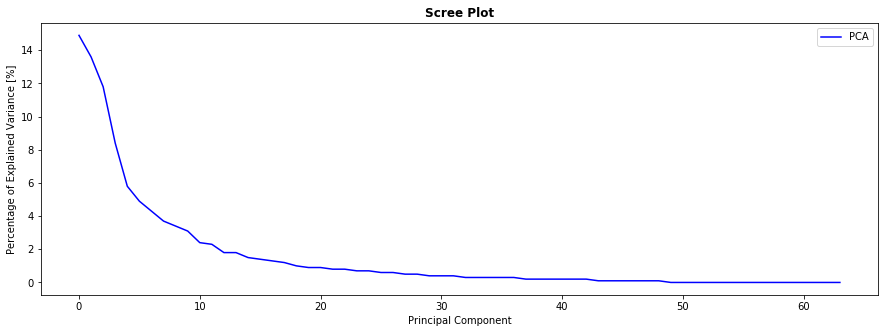
\includegraphics[width = 0.9\textwidth]{figures/pca_handwritten_digits_scree.png}
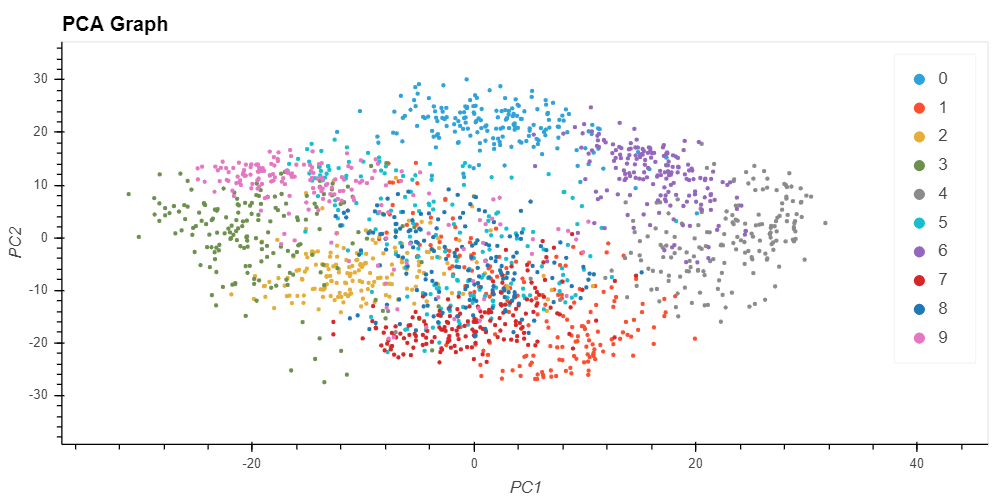
\includegraphics[width = 0.9\textwidth]{figures/pca_handwritten_digits.png}
\end{figure}
\end{frame}

%----------------------------------------------------------------------------------------
%	Fundamentals
%----------------------------------------------------------------------------------------

\section{Fundamentals}

\subsection{Regression}
\subsection{Sparsity inducing Norms}

%----------------------------------------------------------------------------------------
%	Sparse Principal Component Analysis
%----------------------------------------------------------------------------------------

\section{Sparse PCA}

\subsection{Mathematical Formulation}
\subsection{Numerical Solution}

\begin{frame}
\begin{algorithm}[H]
  \scriptsize
    \caption{General SPCA Algorithm}
    \begin{algorithmic}[1]
        \Procedure{SPCA}{$A,B$}
        	\State $\mat A \gets \mat V[,1 \colon k]$, the loadings of the first k ordinary principal components
            \While{not converged} \Comment{Definiere Abbruchkriterium}
                \State Given a fixed $\mat A = [\alpha_1, \ldots, \alpha_k]$, solve the elastic net problem $$\beta_j = \argmin_{\beta} \norm{\mat X \alpha_j - \mat X \beta}^{2} + \lambda \norm{\beta}^2 + \lambda_{1,j}\norm{\beta}_{1}$$
                \State For a fixed $\mat B = [\beta_1, \ldots, \beta_k]$, compute the SVD of $$\mat X^T \mat X \mat B = \mat U \mat D \mat V^T$$
                \State $\mat A \gets \mat U \mat V^T$
            \EndWhile
            \State $\hat{V}_j = \frac{\beta_j}{\norm{\beta_j}}$ for $j = 1, \ldots, k$
        \EndProcedure
    \end{algorithmic}
\end{algorithm} 
\end{frame}

\subsection{Adjusted Variances}
\subsection{p >> n case}

%----------------------------------------------------------------------------------------
%	Application
%----------------------------------------------------------------------------------------

\section{Application}

\subsection{Dataset}
\subsection{Results}

%----------------------------------------------------------------------------------------
%	References
%----------------------------------------------------------------------------------------

\section{References}
\begin{frame}

\frametitle{References}

\begin{thebibliography}{9}
\bibitem[Beamerpaket]{paket} \emph{Beamer Paket} \\ 
\text{http://latex-beamer.sourceforge.net/}
\bibitem[Beamerdokumentation]{doku} \emph{User's Guide to the Beamer} 
\bibitem[Dante]{dante} \emph{DANTE e.V.} \text{http://www.dante.de}   
\end{thebibliography}


\end{frame}


\section{Appendix}

\end{document}
